% !TEX root = index.tex

\section{Principal Curvatures}

\epigraph{If you are receptive and humble, mathematics will lead you by the hand.}{Paul Dirac}

For the graph $z=f(x,y)$ the Gaussian and Mean curvatures are the determinant and trace of $\hess(f)$ respectively, and are invariant under rotation of the $xy$-plane. We can ask: how much can we simplify $\hess(f)$ by replacing it with a suitable $P^{-1} \hess(f) P$?\\ Answer: A Lot.\\

The Hessian $ \hess(f)$ is a symmetric $ 2 \times 2$ matrix, hence by the \textbf{Spectral Theorem}, there exist orthonormal vectors (eigenvectors) $ v_1, v_2$ and constants (eigenvalues) $ \kappa_1, \kappa_2$ such that for the matrix $ P$ whose columns are $v_1, v_2$ we have
\begin{align}
	P^{-1} \hess(f) P  = \begin{bmatrix} \kappa_1 & \\ & \kappa_2 \end{bmatrix}
\end{align}
The set $\{ \kappa_1, \kappa_2 \}$ is uniquely determined by $\hess(f)$.

\begin{definition}
	The eigenvalues $ \kappa_1, \kappa_2$ of $ A$ are called the \textbf{principal curvatures} and the eigenvectors $ v_1, v_2$ are called the \textbf{principal directions} at $p$.
\end{definition}
\begin{remark}
	In the case $ \kappa_1 = \kappa_2$ all directions are principal.
\end{remark}
\begin{ques}
	Show that the various curvatures are related as follows:
	\begin{align}
		\nonumber H &= (\kappa_1 + \kappa_2)/2 \\
		\nonumber K &= \kappa_1 \kappa_2 \\
			\label{eq:eigenvalues}
		&\kappa_1, \kappa_2 \mbox{ are the roots of } \kappa^2 - 2H \kappa + K
	\end{align}
\end{ques}
\begin{ques}
	Find the Principal Curvatures and Principal Directions of the curves you analyzed yesterday
	\begin{description}
		\item[The Perfect \textbf{Potato Chip}: ]  $ z = x^2 - y^2 $
		\item[Cylindrical Potato: ] $z = -\sqrt{r^2 - x^2} $
		\item[Spherical Potato: ] $z = -\sqrt{r^2 - x^2 - y^2}$
		\item[Parabolic Cylinder: ] $z =  x^2$
	\end{description}
	(You can use the estimate $-\sqrt{r^2 - \alpha} \approx -r + \frac{\alpha}{2r} $.)
\end{ques}
\noindent This is all the algebra we'll be needing. We'll now start analyzing the curvatures geometrically.



% \subsection{Principal Curvatures as Good Approximations}
% We can rotate the $xy$-plane about the $z$-axis so that the two axes now point in the direction of the vectors $v_1$ and $v_2$. Without loss of generality let us assume that $v_1$, $v_2$ point in the $x, y$ direction to begin with. Then the Hessian becomes
% \begin{alignat*}{4}
% \hess(f) = &	\begin{bmatrix}
% 		f_{xx} & f_{xy} \\
% 		f_{xy} & f_{yy}
% 	\end{bmatrix} & \quad = \quad &
% 	\begin{bmatrix}
% 		\kappa_1 & 0         \\
% 		0         & \kappa_2
% 	\end{bmatrix}                                                   \\
% 	\Rightarrow \quad &
% 	f(x, y)                & \approx \quad & f(p) + \kappa_1 \cdot \dfrac{x^2}{2} + \kappa_2 \cdot \dfrac{y^2}{2}
% \end{alignat*}
% We've seen such expressions before. The right hand side is the quadratic approximation of the function
% \begin{align*}
% 	f(x,y) &= \sqrt{ f(p)^2 - }
% \end{align*}
%
% This is the geometric significance of the principal directions and principal curvatures:
% \begin{prop}
% 	\label{thm:principal_curvatures}
% 	If $ \kappa_1, \kappa_2 $ are the principal curvatures of the graph of $f(x,y)$ at a critical point $ p$ then near $ p$, after possibly rotating the $xy$-plane about the $z$-axis, the quadratic function that \textbf{best approximates} $f$ is
% 	\begin{align*}
% 		f(p) + \kappa_1\dfrac{x^2}{2} + \kappa_2\dfrac{y^2}{2}
% 	\end{align*}
% \end{prop}
% This is completely analogous the situation in one variable where the circle of radius $1/\kappa$ provided a best approximation for a curve. In 2 dimensions, it's not enough to look at circles alone instead we need to allow for 2 variables {\color{red}something}.
%
% \begin{ques}
% 	For the graph $ z =f(x,y)$ show that the equation of the tangent plane at $ p = (0,0)$ is given by
% 	\begin{align*}
% 		z = f(p) + f_x(p) x + f_x(p) y
% 	\end{align*}
% 	Compare this to Proposition \ref{thm:principal_curvatures}.
% \end{ques}




\begin{figure}[H]
	\centering
	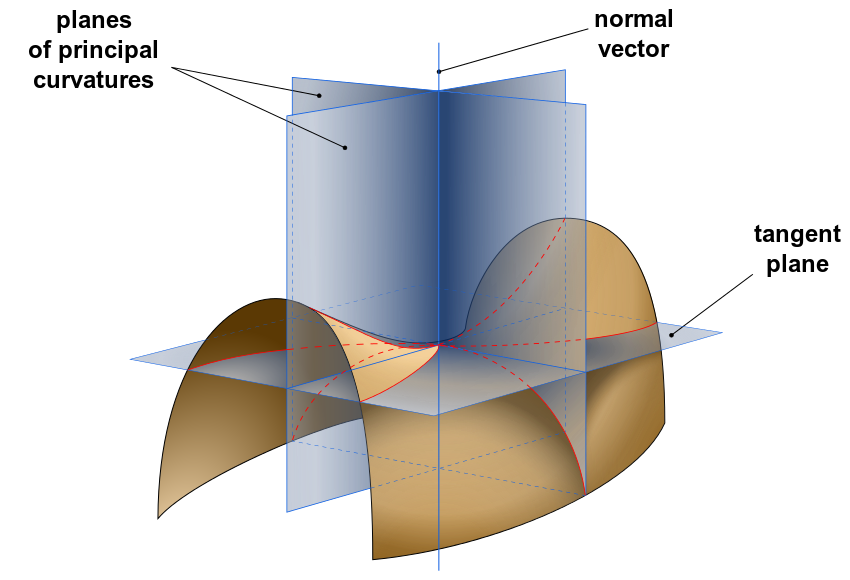
\includegraphics[width=8cm]{normal_curvature}
	\caption{Principal Directions and Normal Curvatures. Image from Wikipedia.}
\end{figure}

\subsection{Curves on a Potato}
Without any loss of generality assume that the $x, y$ axes are the principal directions with principal curvatures $\kappa_1$, $\kappa_2$ respectively. This is equivalent to saying that the degree 2 Taylor approximation of $ f$ is
\begin{align*}
	f(x,y) &\approx f(0,0) + \kappa_1 \cdot \dfrac{x^2}{2} + \kappa_2 \cdot \dfrac{y^2}{2}
\end{align*}
Let us look at the \emph{curves on the surface} passing through $(0,0)$ and compute their curvature in terms of $ \kappa_1, \kappa_2$. We'll consider curves of the form
\begin{align*}
	c_\theta(t)
	 & = (t \cos \theta, t \sin \theta, f(t\cos \theta,t\sin \theta))
\end{align*}
Note that upon projecting onto the $xy$-plane $c_\theta(t)$ projects onto the straight line $y=\tan \theta \cdot x$. Applying the formula for curvature we get:
\begin{align*}
	c'_\theta(t) &= (\cos \theta, \sin \theta, f'(t\cos \theta,t\sin \theta) \\
	c''_\theta(t) &= (0, 0, f''(t\cos \theta,t\sin \theta))
\end{align*}
Because $c(0)=(0,0)$ is the critical point, the tangent plane to $S$ at $(0,0)$ is horizontal and hence we must have $f'(t\cos \theta,t\sin \theta)|_{t=0}=0$ so that
\begin{align*}
	c'_\theta(0) &= (\cos \theta, \sin \theta, 0)
\end{align*}
which is unit length. By explicitly computing the cross product we get
\begin{align*}
	\kappa
	&= |c''_\theta \times c'_\theta|_{t=0} \\
	&= |f''(t\cos \theta,t\sin \theta)|_{t=0}
\end{align*}
We'll remove the absolute value $\lvert - \rvert$ and compute the \textbf{signed curvature}
\begin{align*}
	\kappa &= f''(t\cos \theta,t\sin \theta)|_{t=0}
\end{align*}
\begin{definition}
	\label{def:normal_curvature}
	The signed curvature of $c_\theta(t)$ at $t=0$ is called the \textbf{normal curvature} at $p$ along the direction $(\cos \theta, \sin \theta)$ (we will abbreviate this as just the direction $\theta$).
\end{definition}
We can compute this using the Taylor approximation
\begin{align*}
	f(t\cos \theta,t\sin \theta) &\approx f(0,0) + \kappa_1 \cdot \dfrac{(t \cos \theta)^2}{2} + \kappa_2 \cdot \dfrac{(t \sin \theta)^2}{2} + \cdots \\
	\Rightarrow \qquad
	f''(t\cos \theta,t\sin \theta) &\approx  \kappa_1 \cdot \cos^2 \theta + \kappa_2 \cdot \sin^2 \theta + \cdots
\end{align*}
When we plug in $t=0$ the higher degree terms in the Taylor approximation vanish and we get
\begin{align*}
	\kappa = f''(t\cos \theta,t\sin \theta)|_{t=0} &=  \kappa_1 \cdot \cos^2 \theta + \kappa_2 \cdot \sin^2 \theta
\end{align*}

\begin{prop}
	With the notation as above, the normal curvature at the point $p$ in the direction $\theta$ equals
	  \begin{align*}
			\kappa &=  \kappa_1 \cdot \cos^2 \theta + \kappa_2 \cdot \sin^2 \theta
	  \end{align*}
\end{prop}

\begin{thm}
	\label{thm:extremal_curvatures}
	Without any loss of generality assume that $\kappa_1 \ge \kappa_2$. Then the maximum and minimum normal curvatures at the point $p$ are $\kappa_1$ and $\kappa_2$ respectively, in the corresponding principal directions.
\end{thm}
\noindent Proof is in the following exercise.
\begin{ques}
	Assume $\kappa_1 \ge \kappa_2$. Prove that $\kappa_1 \cos^2 \theta  + \kappa_2 \sin^2 \theta$ attains it maximum at $ \theta = 0, \pi$ and minimum at $ \theta = \pi/2, 3 \pi/2$ and the maximum value is $ \kappa_1$ and the minimum value is $ \kappa_2$.
\end{ques}
\begin{ques} There is another sense in which the Mean Curvature is the mean: it is the mean of all normal curvatures.
	\begin{enumerate}
		\item Plot $ r=\kappa_1 \cos^2 \theta  + \kappa_2 \sin^2 \theta$ in polar coordinates. Interpret this geometrically.
		\item Show that
		\begin{align*}
			H = \dfrac{1}{2 \pi} \int \limits_{0}^{2 \pi } \kappa_1 \cos^2 \theta  + \kappa_2 \sin^2 \theta \: d \theta
		\end{align*}
	\end{enumerate}
\end{ques}
\begin{remark}
	Because curvature does not change when we rotate $\R^3$ we can drop the condition that $p$ is a critical point from the above theorem. It is worth rephrasing the theorem to state this.
\end{remark}
\begin{thm}
	At every point $p$ on a surface $S$ there are two perpendicular directions (principal directions) along which the normal curvatures attain the maximum and minimum (principal curvatures).
\end{thm}

\subsection{Classification of Points}
The signs of the principal curvatures allow us to classify the points on the surface.
\begin{figure}[H]
	\centering
\begin{tabular}{|l|l|l|}
	\hline
	& the surface looks like a ... & such points are called ...\\ \hline
	$\kappa_1, \kappa_2 $ both positive/negative & ellipsoid &  elliptic \\ \hline
	$\kappa_1, \kappa_2$ have opposite signs & hyperboloid & hyperbolic \\ \hline
	$\kappa_1 \kappa_2 = 0$ & cylinder/plane & parabolic \\\hline
\end{tabular}
\end{figure}
\begin{figure}[H]
  \centering
  \begin{subfigure}[t]{0.30\textwidth}
    \centering
    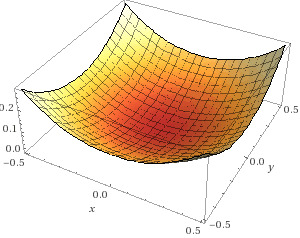
\includegraphics[width=4cm]{sphere}
    \caption{$ K > 0$}
  \end{subfigure}
	\begin{subfigure}[t]{0.30\textwidth}
    \centering
    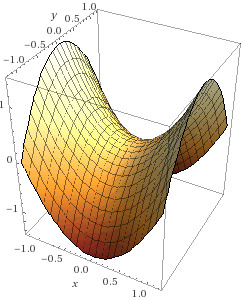
\includegraphics[width=3cm]{wafer}
    \caption{$ K < 0 $}
  \end{subfigure}
	\begin{subfigure}[t]{0.30\textwidth}
    \centering
    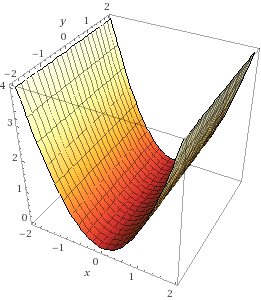
\includegraphics[width=3cm]{parabola1}
    \caption{$K = 0$}
  \end{subfigure}
\end{figure}
Note that because $K = \kappa_1 \kappa_2$ the above three classifications are essentially the classifications based on Gaussian curvature. This already suggests that the Gaussian curvature sees some \emph{intrisic} curvature of surfaces.\\

\begin{ques}
	Classify the points on a torus as elliptic, hyperbolic, or parabolic.
	\begin{figure}[H]
    \centering
    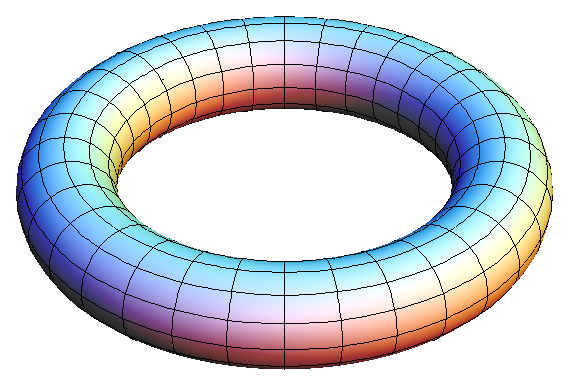
\includegraphics[width=10cm]{torus}
  \end{figure}
\end{ques}

\newpage
\subsection{Appendix: Spectral Theorem}
A basis $ v_1, v_2, \cdots, v_n$ of $ \R^n$ is said to be \textbf{orthonormal} if $ \norm{v_i}=1 $ for each $ i$ and $ v_i \cdot v_j = 0$ for $ i \neq j$.

\begin{thm}[Spectral Theorem for Symmetric Matrices]
	Let $ A$ be a \textbf{symmetric} $ n \times n$ matrix with real entries. Then there exists an orthonormal basis $ v_1, v_2, \cdots, v_n$ basis of $ \R^n$ and real numbers $ \kappa_i$ such that
	\begin{align*}
		A v_i = \kappa_i v_i
	\end{align*}
	Equivalently, if $P$ is the matrix with columns $ v_i$ then
	\begin{align*}
		P^{-1} A P =
		\begin{bmatrix} \kappa_1 &           &        &           \\
			          & \kappa_2 &        &           \\
			          &           & \ddots &           \\
			          &           &        & \kappa_n
		\end{bmatrix}
	\end{align*}
	The $ \kappa_i$ (\textbf{eigenvalues}) are unique up to permutations and the orthonormal basis $ v_1, v_2, \cdots, v_n$ (\textbf{eigenvectors}) and the matrix $ P$ are `essentially' unique.
\end{thm}
The following exercise outlines the proof for $n=2$.


\begin{ques}
	Consider the symmetric matrix $A = \begin{bmatrix} a & b \\ b & c\end{bmatrix}$. Assume that $A$ is not a scalar matrix i.e. $A \not= \begin{bmatrix} a & 0 \\ 0 & a\end{bmatrix}=aI$ (this case is trivial).
	\begin{enumerate}
		\item Show that the equation
		\begin{align*}
			\det(A - \kappa I) = \det \begin{bmatrix} a -\kappa & b \\ b & c - \kappa \end{bmatrix} = 0
		\end{align*}
		has 2 distinct real solutions $\kappa_1, \kappa_2$.
		\item Argue that there exist 2 linearly independent unit length vectors $v_1, v_2$ satisfying
		$ A v_i = \kappa_i v_i$
		for $i = 1, 2$.\hint{Look at the kernel of $A - \kappa_i I$.}
		\item Prove that $v_1 \perp v_2$.\hint{Find $v_1 ^ T A v_2$ in 2 different ways.}
	\end{enumerate}
	Let $P$ be the matrix with column vectors $v_1, v_2$.
	\begin{enumerate}[resume]
		\item Prove that $P^T = P^{-1}$.
		\item By an explicit computation show $P^T A P = \begin{bmatrix} \kappa_1 & 0 \\ 0 & \kappa_2 \end{bmatrix}$
	\end{enumerate}
\end{ques}
